\ifx\FORMAT\undefined
\documentclass[11pt]{book}
\usepackage{amsmath,mathtools}
\usepackage[utf8]{inputenc}
\usepackage[ngerman]{babel}
\usepackage[T1]{fontenc}
\usepackage{lmodern}
\usepackage{acronym}
\usepackage{graphicx} 
\usepackage{epstopdf}
\usepackage{svg}
\usepackage{multirow}
\usepackage{amssymb}
\usepackage{trfsigns}
\usepackage{setspace}
\usepackage{yfonts}
\usepackage{nomencl}
\usepackage{float}
\usepackage{subfig}
\usepackage{scrpage2}
\usepackage{afterpage}
\usepackage{longtable}

\onehalfspacing


%Hyperlinks package, links aus inhaltsverzeichnis
\usepackage{hyperref}
\hypersetup{
    colorlinks=false, %set true if you want colored links
    linktoc=all,
    linkbordercolor = {white},
    citecolor = {white},
    allbordercolors = {white},
}
%Blattformatierung
\usepackage{geometry}
\geometry{a4paper, top=25mm, left=30mm, right=25mm, bottom=20mm}

%Listing
\usepackage{courier}
\usepackage{listings}
\usepackage{color}
 \lstset{
   frame=tb,
   framexleftmargin=2.5em,
   basicstyle=\small\linespread{0.9}\bfseries\ttfamily,
   emph={square}, 
   emphstyle=\color{blue}\texttt,
   emph={[2]root,base},
   emphstyle={[2]\color{yac}\texttt},
   showstringspaces=false,
   flexiblecolumns=false,
   tabsize=2,
   numbers=left,
   numberstyle=\small\bfseries\ttfamily,
   numberblanklines=false,
   stepnumber=1,
   numbersep=10pt,
   xleftmargin=25pt
 }
 
 \def\presuper#1#2%
	{\mathop{}%
	\mathopen{\vphantom{#2}}^{#1}%
	\kern-\scriptspace%
	#2}
%Display vecotr in a reference frame
\newcommand{\vecBS}[4]{\presuper{#1}{\begin{pmatrix}
#2 \\ #3 \\ #4
\end{pmatrix}}}
%Boldsymbol shortcut
\newcommand{\bs}[1]{\boldsymbol{#1}}
%Bezugssystemdefinition
\newcommand{\defBS}[1]{\{#1\} [ \bs{e}_{{#1}_1},\bs{e}_{{#1}_2}, \bs{e}_{{#1}_3} ]}
%Projektionsmatrix
\newcommand{\pMat}[2]{\presuper{#1}{\bs{P}}^{#2}}
%Differenation in Respekt zu BS
\newcommand{\diffIn}[3]{\frac{\presuper{#1}{d{#2}}}{d#3}}
\newcommand{\partialDiffIn}[3]{\frac{\presuper{#1}{\partial{#2}}}{\partial #3}}
%Geschwindigkeit/Beschleunigung
\newcommand{\vel}[3]{\presuper{#1}{\bs{#2}}^{#3}}

%Rightarrow with spaceing
\newcommand{\rArrow}{\hspace{5pt}\rightarrow\hspace{5pt}}
%Inneres Produkt
\newcommand{\inProd}[2]{\langle {#1}, {#2} \rangle}
\begin{document}
\fi

\chapter{Reglerentwurf für das Balancieren auf einer Ecke}
Nachdem im vorherigen Kapitel ein Modell des Systems entwickelt wurde muss nun für dieses ein Regler entworfen werden. Hierfür wird zunächst die kontinuierliche Zustandsraumdarstellung in eine diskrete überführt. Anschließend wird diese in eine Kalman-Dekomposition transformiert, um das System auf eine Minimalrealisierung zu reduzieren. Diese besteht lediglich aus steuer- und beobachtbaren Zuständen und kann somit als Ausgangspunkt für den Reglerentwurf genutzt werden. Für die Bestimmung des Reglers wird ebenfalls das LQR-Verfahren verwendet. Der Regler wird im nächsten Schritt an Hand einer Simulation überprüft, wobei der Verlauf der nicht steuerbar bzw. beobachtbaren Zustände untersucht wird. Des weiteren wird mittels der Simulation die Direktionalitätsproblematik des Mehrgrößensystems analysiert, welche durch die Stellgrößenbeschränkungen verursacht wird. Der resultierende Regle wird im Anschluss auf die reelle Strecke übertragen und dort empirisch optimiert.

\newpage
\section{Modell basierter Reglerentwurf}
Aus dem letzten Kapitel ist die Zustandsgleichung
\begin{equation}
\dot{\bs{x}} = \underbrace{\begin{bmatrix}
\bs{0}^{3\times 3} & \Delta\varPhi & \bs{0}^{3\times 3} 
\\
\bs{I}_K^{-1}\cdot\Delta\bs{T}_G & -C_{\psi}\cdot\bs{I}^{-1}_K & C_{\psi}\cdot\bs{I}^{-1}_K
\\
\bs{0}^{3\times 3} & C_{\psi}\cdot\bs{I}^{-1}_R & -C_{\psi}\cdot\bs{I}^{-1}_R
\end{bmatrix}}_{=\bs{A}_c} \cdot \underbrace{\begin{bmatrix}
\bs{\overline{\varphi}} 
\\
\bs{u}_K \\
\bs{u}_R
\end{bmatrix}}_{=\bs{x}}
+
\underbrace{\begin{bmatrix}
\bs{0}^{3\times 3}
\\
-\bs{I}^{-1}_K
\\
\bs{I}^{-1}_R
\end{bmatrix}}_{=\bs{B}_c}\cdot \underbrace{\begin{bmatrix}
T_{M1} \\ T_{M2} \\ T_{M3}
\end{bmatrix}}_{=\bs{u}}
\end{equation}
hervorgegangen. Der Ausgangsvektor $\bs{y}\in \mathcal{R}^8$ enhält alle Zustandsgrößen bis auf den Winkel $\varphi_1$, da dieser nicht aus den Sensordaten ermittelt werden kann.
\begin{equation}
\bs{y} = \underbrace{\begin{bmatrix}
\bs{0}^8 & \bs{I}^{8\times 8}
\end{bmatrix}}_{\equiv \bs{C}_c} \cdot \bs{x}
\end{equation}
Im nächsten Schritt wird das kontinuierliche System \cSS{A_c}{B_c}{C_c} in das diskrete System \dSS{A}{B}{C} überführt. Hierfür wird die Abtastrate $f_a = 50Hz$ verwendet.
Anschließend wird das System mittels der Kalmankriterien auf Steuer- und Beobachtbarkeit geprüft. Hieraus folgt, dass das System sowohl einen nicht steuerbaren als auch einen nicht beobachtbaren Zustand besitzt. Eine Voraussetzung für den Entwurf eines Zustandreglers besteht darin, dass das System vollständig steuer- und beobachtbar ist. Deshalb kann das System \dSS{A}{B}{C} nicht direkt für den Reglerentwurf verwendet werden. Zunächst muss eine Minimalrealisierung \dSS{A_M}{B_M}{C_M} gefunden werden, welche nur den steuer- und beobachtbaren Unterraum des Systems enthält. Um eine Minimalrealisierung des Systems zu erhalten wird es in eine so genannte Kalman-Dekomposition \dSS{A_K}{B_K}{C_K} überführt. Die hierfür nötige Transformationsmatrix $\bs{T}_K$ wird mittels der Matlab-Funktion \textit{minreal()} bestimmt.
\begin{equation}
\bs{x}_K = \bs{T}^{-1}_K\cdot \bs{x}\hspace{25pt} \bs{A}_K = \bs{T}^{-1}_K\cdot \bs{A}\cdot \bs{T}_K \hspace{25pt} \bs{B}_K = \bs{T}^{-1}_K\cdot \bs{B} \hspace{25pt} \bs{C}_K = \bs{C}\cdot \bs{T}_K
\end{equation}
\begin{equation}
\underbrace{\begin{bmatrix}
\bs{x}_M \\ x_{\overline{S}} \\ x_{\overline{B}}
\end{bmatrix}}_{= \bs{x}_K}(k+1) = 
\underbrace{\begin{bmatrix}
\bs{A}_M & \bs{a}_{M/\overline{S}} & 0 \\
\bs{0}^{1\times 7} & a_{\overline{S}} & 0 \\
\bs{a}_{\overline{B}/M} & a_{\overline{B}/\overline{S}} & a_{\overline{B}}
\end{bmatrix}}_{= \bs{A}_K}\cdot \begin{bmatrix}
\bs{x}_M \\ x_{\overline{S}} \\ x_{\overline{B}}
\end{bmatrix}(k) + 
\underbrace{\begin{bmatrix}
\bs{B}_M \\ \bs{0}^{1\times 3} \\ \bs{b}^{T}_{\overline{B}}
\end{bmatrix}}_{=\bs{B}_K}\cdot \bs{u}(k)
\end{equation}
\begin{equation}
\bs{y}(k) = \underbrace{\begin{bmatrix}
\bs{C}_M  & \bs{c}_{\overline{S}} & \bs{0}^8
\end{bmatrix}}_{=\bs{C}_K}\cdot \bs{x}_K(k)
\end{equation}
Die Kalman-Dekomposition \textfrak{D}$_K$($\bs{A}_K$,$\bs{B}_K$,$\bs{C}_K$) setzt sich aus der Minimalrealisierung \textfrak{D}$_M$($\bs{A}_M$,$\bs{B}_M$,$\bs{C}_M$, dem nicht steuerbaren Teilsystem \textfrak{D}$_{\overline{S}}$($a_{\overline{S}}$,$\bs{0}^{3\times 1}$,$\bs{c}_{\overline{S}}$) und dem nicht beobachtbaren Teilsystem \textfrak{D}$_{\overline{B}}$($a_{\overline{B}}$,$\bs{b}^T_{\overline{B}}$,$\bs{0}^{8\times 1}$) zusammen.\footnote{Die hier gezeigt Dekomposition stellt nicht den allgemein gültigen Fall dar, der ein weiteres Teilsystem weder steuer- noch beobachtbaren Zustände enthält [Lunze RT2, S.108ff]} Prinzipiell kann nun für das System \textfrak{D}$_M$ ein Zustandsregler entwickelt werden, der zu einem asymptotischen System führt. Allerdings ist dabei zu beachten, dass die Teilsysteme \textfrak{D}$_M$, \textfrak{D}$_{\overline{S}}$ und \textfrak{D}$_{\overline{B}}$ nicht voneinander entkoppelt sind. Die Abhängigkeiten zwischen den Teilsystemen werden von den den Größen $\bs{a}_{M/\overline{S}}$, $\bs{a}_{\overline{B}}/M$ und $a_{\overline{B}/\overline{S}}$ beschrieben. Da der Zustandsregler lediglich die Eigenwerte des Teilsystem \textfrak{D}$_M$ beeinflussen kann, muss zusätzlich die Stabilität der Teilsysteme \textfrak{D}$_{\overline{S}}$ und \textfrak{D}$_{\overline{B}}$ geprüft werden. In diesem Kontext wird der Begriff der Stabilisierbarkeit verwendet, wobei ein System stabilisierbar heißt wenn all seine Eigenvorgänge, die nicht Teil seines vollständig steuer- und beobachtbaren Unterraums sind, asymptotisch stabil sind. In diesem Anwendungsfall handelt es sich bei \textfrak{D}$_{\overline{S}}$ und \textfrak{D}$_{\overline{B}}$ um Systeme erster Ordnung, derer Eigenwert $\lambda_{\overline{S}}$ bzw. $\lambda_{\overline{B}}$ auf dem Einheitskreis liegt.
\begin{equation}
\lambda_{\overline{S}} = \lambda_{\overline{B}} = 1
\end{equation}
Somit sind die beiden Teilsysteme grenzstabil. Um den Verlauf und Einfluss der Zustände $x_{\overline{S}}$ und $x_{\overline{B}}$ nachzuvollziehen wird zunächst ein Regler für die Minimalrealisierung \textfrak{D}$_M$ entworfen und in einer Simulation erprobt. Für die Bestimmung der Reglermatrix $\bs{K}_M$ wird das LQR-Verfahren angewandt, wobei die Gewichtungsmatrizen $\bs{Q}$ und $\bs{R}$ in Diagonalform gewählt werden. Als Diagonalelemente werden die Kehrwerte der maximal zulässigen Zustandsgrößen im Quadrat verwendet. Hierbei ist zu beachten, dass der Reglerentwurf für das System \textfrak{D}$_M$ durchgeführt wird. Deshalb muss der maximale Zustandsvektor $\bs{x}_{max}$ in dessen Darstellung transformiert werden. Hierfür wird mit der Transformationsmatrix $\bs{T}^{-1}_K$ und einer nicht regulären Reduktionsmatrix multipliziert.
\begin{equation}
\bs{x}_{M,max} = \begin{bmatrix}
\bs{I}^{7\times 7} & \bs{0}^{7\times 2}
\end{bmatrix}\cdot \bs{T}^{-1}_K \cdot \bs{x}_{max}
\label{eq_xred}
\end{equation}
\begin{equation}
\bs{Q} = diag(\bs{x}_{M,max})^{-2} \hspace{35pt} \bs{R} = diag(\bs{u}_{max})^{-2}
\end{equation}
In der Simulation wird für die Regelstrecke das kontinuierliche System \textfrak{S}$_C$($\bs{A}_C$,$\bs{B}_C$,$\bs{C}_C$) verwendet. Für die Implementierung des Reglers ist ebenfalls in (\cite{eq_xred}) beschriebene Transformation nötig.
\begin{equation}
\bs{u}(k) = -\underbrace{\bs{K}_M\cdot \begin{bmatrix}
\bs{I}^{7\times 7} & \bs{0}^{7\times 2}
\end{bmatrix} \cdot \bs{T}^{-1}_K}_{\equiv \bs{K}} \cdot \bs{x}(k)
\end{equation}
Die folgenden Abbildungen zeigen den Verlauf der Zustandsgrößen $\bs{\overline{\varphi}}$, $\bs{u}_K$ und $\bs{u}_R$ sowie der Stellgrößen $\bs{T}_M$ bei dem Anfangszustand
\begin{equation}
\bs{x}(0) = \begin{bmatrix}
0 \\ 0.11 \\ 0.08 \\ \bs{0}^{6\times 1}
\end{bmatrix}\,.
\end{equation}
\begin{figure}[!ht]
\centering
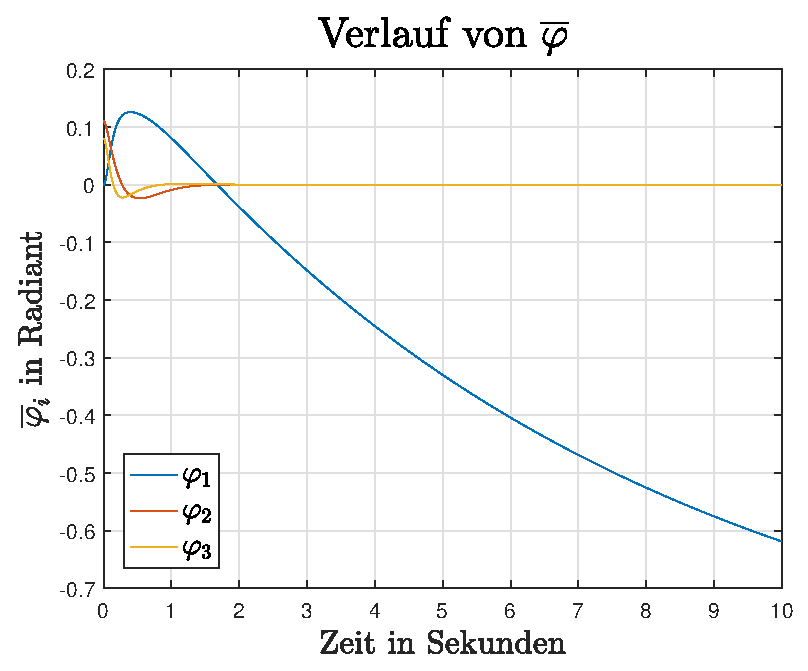
\includegraphics[width=0.45\linewidth]{img/lin_sim1_phi.eps}\hspace{1cm}
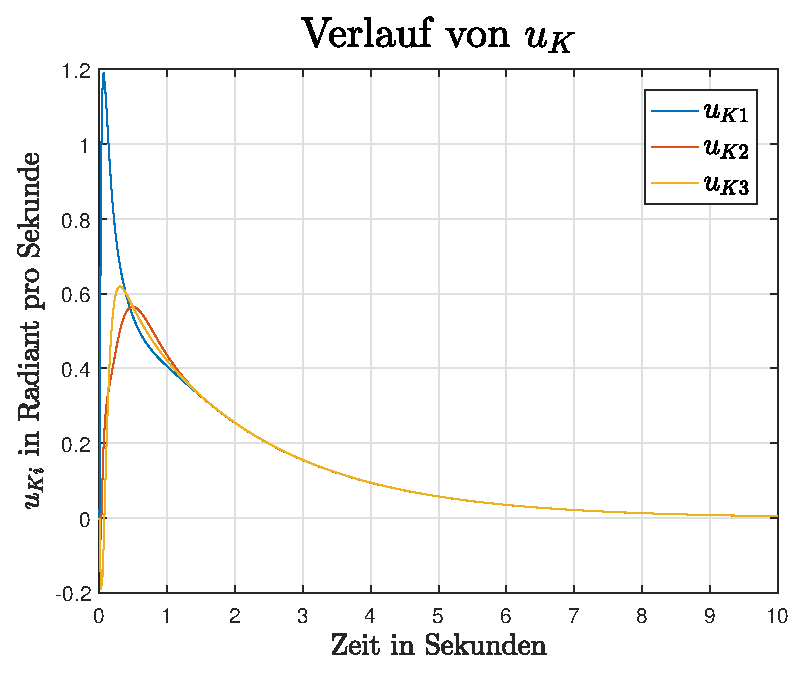
\includegraphics[width=0.45\linewidth]{img/lin_sim1_uk.eps}
\vspace{1cm}

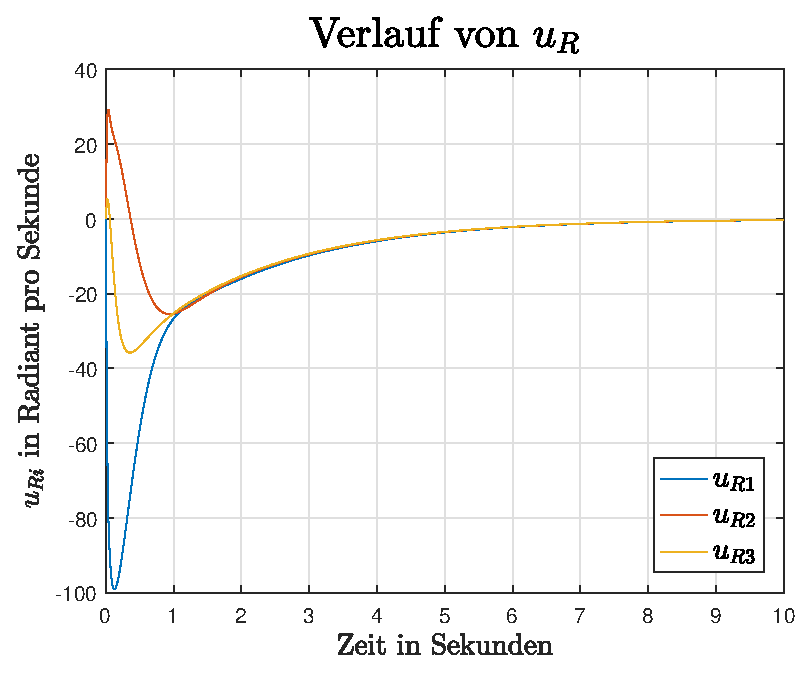
\includegraphics[width=0.45\linewidth]{img/lin_sim1_ur.eps}\hspace{1cm}
\includegraphics[width=0.45\linewidth]{img/lin_sim1_tm.eps}
\end{figure}
Die Simulation zeigt, dass alle Zustandsgrößen bis auf den Winkel $\varphi_1$ gegen null konvergieren. Folglich ist anzunehmen, dass der Zustand $\varphi_1$ nicht teil der Minimalrealisierung \textfrak{D}$_M$ ist. Diese Vermutung lässt sich mittels der Matrizen $\bs{C}_C$ und $\bs{A}_C$ bestätigen. Die erste Spalte der Matrix $\bs{C}_C$ ist ein Nullvektor und somit beeinflusst $\varphi_1$ den Ausgangsvektor $\bs{y}$ nicht. Eine solche Zustandsvariable wird auch als nicht ausgangsverbunden bezeichnet. Des weiteren hat der Zustand $\varphi_1$ keine Auswirkung auf die Systemdynamik. Dies ist auf die erste Spalte der Systemmatrix $\bs{A}_C$
\begin{equation}
\bs{A}_C(:,1) = \begin{bmatrix}
\bs{0}^{3\times 1} \\ \left[\bs{I}^{-1}_K\cdot \Delta\bs{T}_G\right](:,1)\\ \bs{0}^{3\times 1}
\end{bmatrix} = \bs{0}^{9\times 1}
\end{equation}
zurückzuführen, welche ebenfalls ein Nullvektor ist. Hieraus lässt sich schließen, dass es sich bei dem Winkel $\varphi_1$ um den nicht beobachtbaren Zustand $x_{\overline{B}}$ handelt. Dies wird auch von der Struktur der inversen Transformationsmatrix
\begin{equation}
\bs{T}^{-1}_K = \begin{bmatrix}
\bs{0}^{8\times 1} & \bs{T}^{-1}_K(2:9,2:9) \\
1 & \bs{0}^{1\times 8}
\end{bmatrix}
\end{equation}
bestätigt, welche $\varphi_1$ in $x_{\overline{B}}$ abbildet.

Mit Hilfe der Matrix $\bs{T}^{-1}_K$ kann auch der nicht steuerbare Zustand $x_{\overline{S}}$ interpretiert werden. Die zugehörige Zeile
\begin{equation}
\bs{T}^{-1}_K(8,:) \approx \begin{bmatrix}
0 & 0 & 0 & 0,5 & 0,5 & 0,7 & 0,01 & 0,01 & 0,01
\end{bmatrix}
\end{equation}
bildet den Zustandsvektor $\bs{x}$ in die Variable $x_{\overline{S}}$ ab. Diese ist somit eine Linearkombination der Geschwindigkeiten $\bs{u}_K$ und $\bs{u}_R$. Dieser Umstand erklärt auch das asymptotische Verhalten des Zustandvektors in der vorherigen Simulation. Da $\bs{u}_K(0)=\bs{u}_R(0)=\bs{0}$ und somit $x_{\overline{S}}(0)=0$ galt, kam die Grenzstabilität des nicht steuerbaren Zustandes nicht zum Tragen. Wird der Anfangszustand $\bs{x}(0)$ so angepasst, dass $x_{\overline{S}}(0)\neq \bs{0}$ gilt, ergibt sich das folgende Simulationsergebnis.
\clearpage
\begin{figure}[h]
\centering
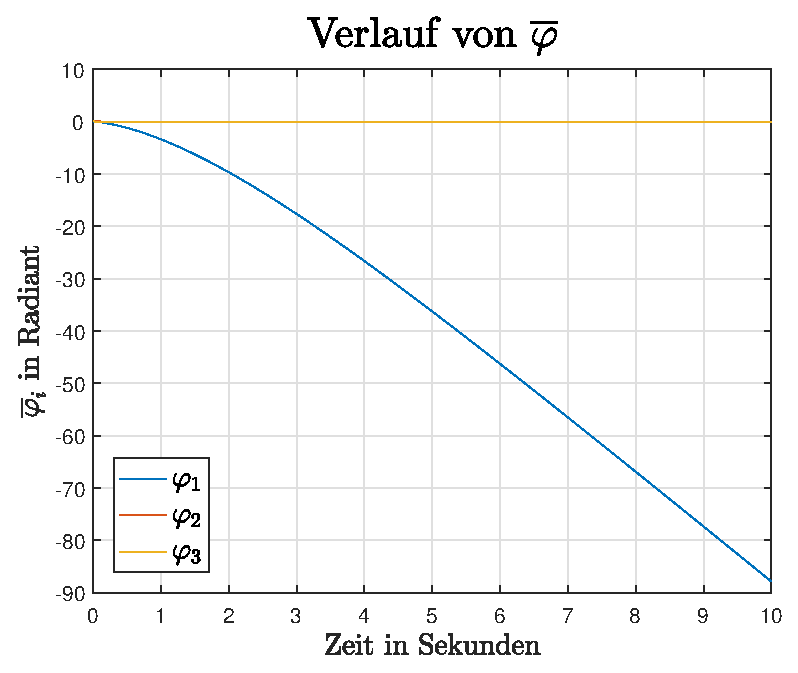
\includegraphics[width=0.45\linewidth]{img/lin_sim2_phi.eps}\hspace{1cm}
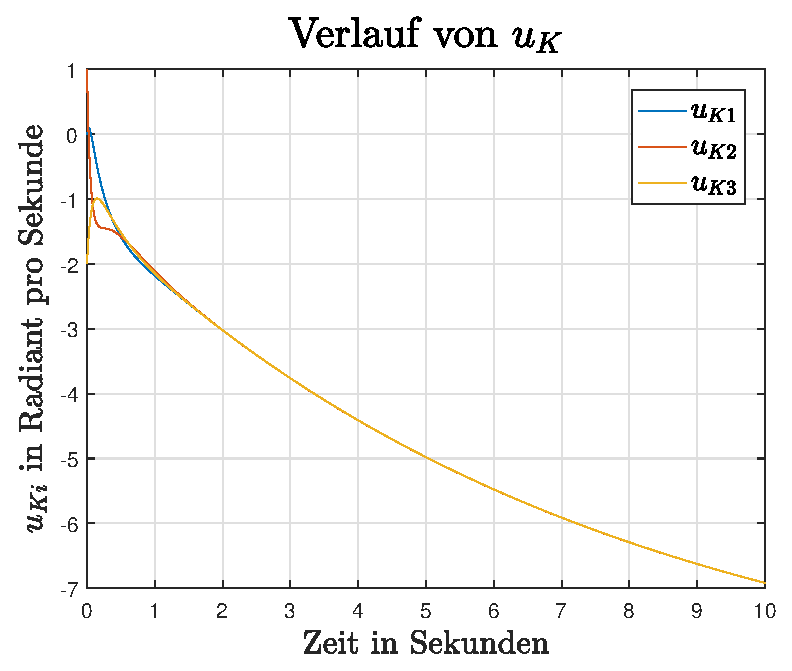
\includegraphics[width=0.45\linewidth]{img/lin_sim2_uk.eps}
\vspace{1cm}

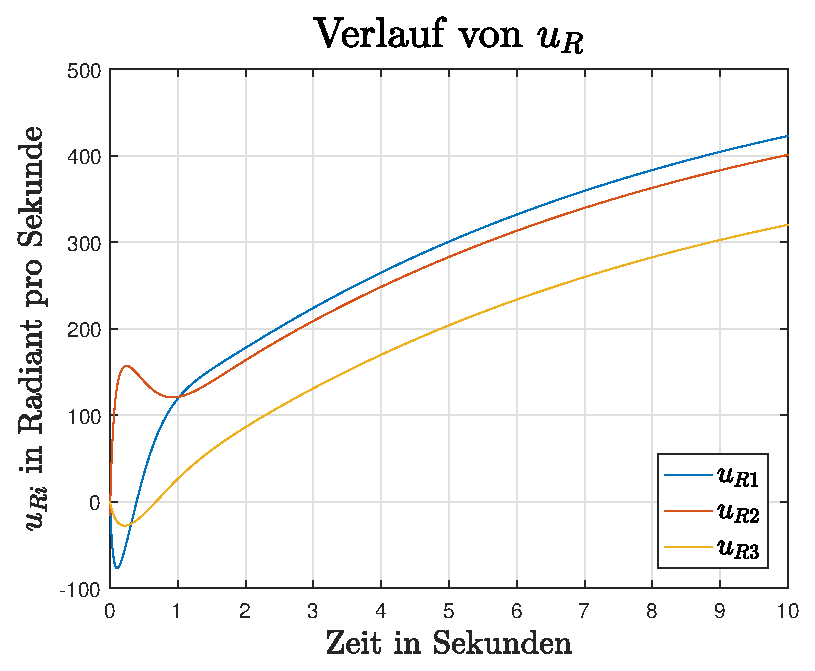
\includegraphics[width=0.45\linewidth]{img/lin_sim2_ur.eps}\hspace{1cm}
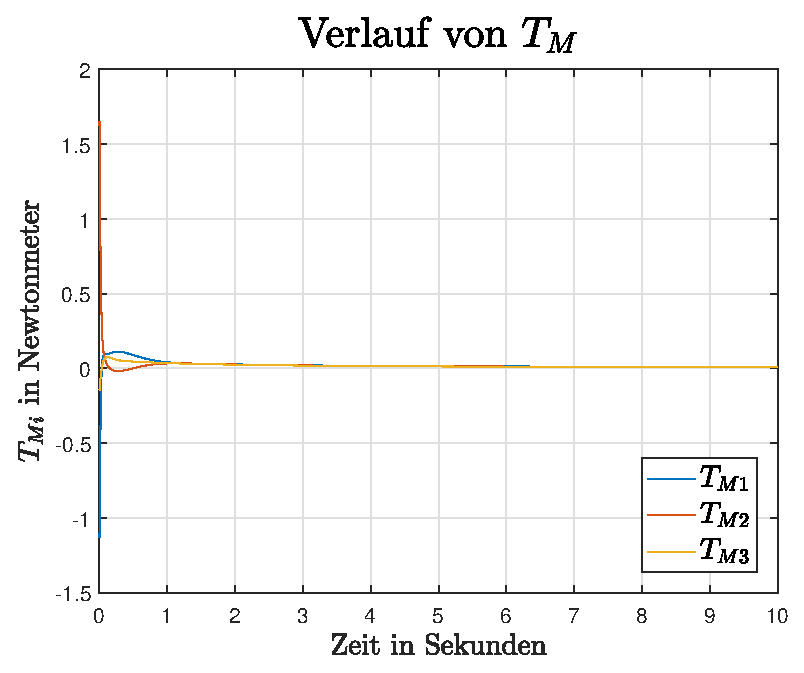
\includegraphics[width=0.45\linewidth]{img/lin_sim2_tm.eps}
\end{figure}
Die Simulation zeigt, dass die Winkel $\varphi_2$ und $\varphi_3$ nach wie vor asymptotisch stabil sind. Allerdings konvergieren die Winkelgeschwindigkeiten $\bs{u}_K$ gegen den gleichen Endwert $u_{Ke}\neq 0$. Mittels der Winkelgeschwindigkeit
\begin{equation}
\vel{A}{\omega}{K} = \vecBS{K}{u_{K1}}{u_{K2}}{u_{K3}}
\end{equation}
bedeutet der Endwert $u_{Ke}$, dass der Würfel mit einer konstanten Winkelgeschwindigkeit um seine Hauptdiagonale rotiert. Ebenso konvergieren die Geschwindigkeiten der Schwungmasse $\bs{u}_R$ und die Stellgrößen gegen einen von Null verschiedenen Endwert. Dieser Umstand kann an Hand des Systems \textfrak{D}$_K$ erklärt werden. Der Unterraum \textfrak{D}$_M$ ist im geschlossenen Regelkreis asymptotisch stabil. Allerdings wirkt der nicht steuerbare Zustand $x_{\overline{S}}$ proportional zu dem Vektor $\bs{a}_{M/\overline{S}}$ auf $\bs{x}_M$ ein.
\begin{equation}
\bs{x}_M(k+1) = \left(\bs{A}_M-\bs{B}_M\cdot \bs{K}_M\right)\cdot \bs{x}_M(k) + \bs{a}_{M/\overline{S}}\cdot \sigma(t)\cdot x_{\overline{S}}(0)
\end{equation}
Mit Hilfe des Endwertsatzes kann das Konvergenzverhalten bestimmt werden.
\begin{equation}
\begin{split}
z\cdot \bs{X}_M(z) &= \left(\bs{A}_M - \bs{B}_M\cdot \bs{K}_M\right)\cdot \bs{X}_M(z)  + \bs{a}_{M/\overline{S}}\cdot X_{\overline{S}}(z)
\\
\leftrightarrow \bs{X}_M(z) &= \left[z\cdot \bs{I} - \left(\bs{A}_M - \bs{B}_M\cdot \bs{K}_M\right) \right] ^{-1} \cdot \bs{a}_{M/\overline{S}}\cdot \underbrace{X_{\overline{S}}(z)}_{= \frac{z}{z-1}\cdot x_{\overline{S}}(t=0)}
\end{split}
\end{equation}
\begin{equation}
\lim_{k\rightarrow\infty} \bs{x}_M(k) = \lim_{z\rightarrow 1}(z - 1)\bs{X}_M(z) \equiv\bs{x}_{M,end}
\end{equation}
Wird der Zustandsvektor $\bs{x}_{K,end}$ aus den Endwerten der Teilsysteme zusammengesetzt kann dieser in den ursprünglichen Zustandsraum transformiert werden.
\begin{equation}
\begin{split}
\bs{x}_{end} &= \bs{T}_K\cdot \begin{bmatrix}
\bs{x}_{M,end} \\ x_{\overline{S}} \\ x_{\overline{B}}
\end{bmatrix} 
\\
&= \begin{bmatrix}
\varphi_1 & 0 & 0 & 5{,}4 x_{\overline{S}} & 5{,}4 x_{\overline{S}} & 5{,}4x_{\overline{S}} & -306{,}9 x_{\overline{S}} & -298{,}2 x_{\overline{S}} & -272{,}1 x_{\overline{S}}
\end{bmatrix}^T
\end{split}
\end{equation}
Dieses Ergebnis besagt, dass das System des Würfels ein Ruhelagenkontinuum besitzt. Die Winkel $\overline{\varphi}_2$ und $\overline{\varphi}_3$ konvergieren stets gegen null, was der aufrechten Position des Würfels auf einer Ecke entspricht. Allerdings rotiert der Würfel dabei mit einer konstanten, von $x_{\overline{S}}$ abhängigen Geschwindigkeit um seine Raumdiagonale. Des weiteren rotieren die drei Schwungmassen mit einer konstanten Endgeschwindigkeit, welche ebenfalls von $x_{\overline{S}}$ abhängt. In diesem Zusammenhang kann auch die nicht Steuerbarkeit des Zustandes $x_{\overline{S}}$ erklärt werden. Angenommen der Würfel rotiert in einer Ruhelage des Kontinuums mit einer konstanten Winkelgeschwindigkeit
\begin{equation}
\vel{A}{\omega}{K} = \vecBS{K}{u_{end}}{u_{end}}{u_{end}}\,.
\end{equation}
Nun ist es zwar möglich diese Rotation durch ein parallel gerichtetes Motormoment
\begin{equation}
\bs{T}_M = \vecBS{K}{T}{T}{T}
\end{equation}
zu beeinflussen, allerdings werden dadurch zwangsläufig die Winkelgeschwindigkeiten $\bs{u}_R$ der Schwungmassen beeinflusst. Somit ist es nicht möglich die Rotation des Würfels um seine Raumdiagonale unabhängig von der Bewegung der Schwungmassen zu beeinflussen, was wiederum gegen die Forderung der vollständigen Steuerbarkeit eines Systems verstößt. Dieses Ergebnis ist kritisch zu betrachtet, da hier lediglich ein linearisiertes System untersucht wurde. Um eine finale Aussage über die Steuerbarkeit des Systems zu treffen, müssen dessen nicht lineare Bewegungsgleichung auf geprüft werden. Da es sich bei dem Würfel um ein eingangslineares System handelt ist dessen Prüfung auf Steuerbarkeit analytisch möglich [Adamy, S.155ff]. Diese Untersuchung wird in dieser Arbeit allerdings nicht durchgeführt, da an der realen Regelstrecke lediglich Anfangszustände mit
\begin{equation}
\bs{\overline{\varphi}} \neq \bs{0} \hspace{35pt} \bs{u}_K \approx \bs{0} \hspace{35pt} \bs{u}_R \approx \bs{0}
\end{equation}
untersucht werden und der nicht steuerbare Zustand $x_{\overline{S}}$ somit nicht besonders ins Gewicht fällt.

\ifx\FORMAT\undefined
\end{document}
\fi
